\label{chapter:applications}

In this chapter we discuss applications of our improvements to the binary XPFC
model.  To begin we'll discuss an effective equation of motion in the limit
that density change on solidification is small, after which we'll examine the
to process of multi-step nucleation of nanoparticles from solution. To conclude
we'll discuss areas of future application.

%%%%%%%%%%%%%%%%%%%%%%%
\subsection{Dynamics} %
%%%%%%%%%%%%%%%%%%%%%%%

To examine applications of our improvements to the XPFC model we begin 
by considering equations of motion. Following \cite{GREENWOOD11_BINARY},
we use conservative dynamics for both $n(x, t)$ and $c(x, t)$.
%
\begin{gather}
    \f{\partial n(x, t)}{\partial t} = 
        M_n \nabla^2\l(\f{\d \beta \Delta\F / \rho_0}{\d n(x, t)}\r) 
        + \xi_n(x, t), \\ 
    \f{\partial c(x, t)}{\partial t} = 
        M_c \nabla^2\l(\f{\d \beta \Delta \F / \rho_0}{\d c(x, t)}\r)
        + \xi_c(x, t).
\end{gather}
%
These equations of motion are largely phenomenological as, strictly speaking,
there is no reason that the local concentration should be conserved.  This
conservation can be justified in the limit that the total density at a course
grained level does not change significantly between phases. When this is the
case we have $c \equiv \B / \rho \approx \B / \rho_0$ which \textit{is}
conserved.

%%%%%%%%%%%%%%%%%%%%%%%%%%%%%%%%%%%%%%%%%%%%%%%%%%%%%%%%%%%%%
\section{Multistep Nucleation of Nanoparticles in Solution} %
%%%%%%%%%%%%%%%%%%%%%%%%%%%%%%%%%%%%%%%%%%%%%%%%%%%%%%%%%%%%%

{
    \color{ForestGreen} Discuss the interest in this process with reference to 
    papers about multistep nucleation theories. Discuss relevance of nanoparticles
    size and prediction of size (catalyzsis, color, etc... size is the basic relevant
    detail of nanoparticles).
}

\begin{figure}
    \centering
    \begin{subfigure}[b]{0.3\textwidth}
        
\includegraphics[width=\textwidth]{initial}
        \label{fig:initial}
        \caption{}
    \end{subfigure}
    ~
    \begin{subfigure}[b]{0.3\textwidth}
        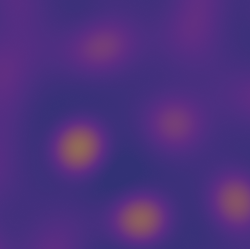
\includegraphics[width=\textwidth]{early_spinodal}
        \label{fig:early_spinodal}
        \caption{}
    \end{subfigure}
    ~
    \begin{subfigure}[b]{0.3\textwidth}
        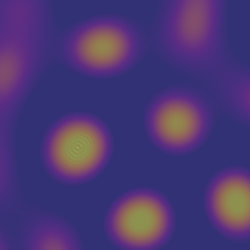
\includegraphics[width=\textwidth]{devel_spinodal.png}
        \label{fig:devel_spinodal}
        \caption{}
    \end{subfigure}

    \vspace{0.5cm}
    \begin{subfigure}[b]{0.3\textwidth}
        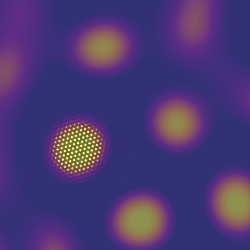
\includegraphics[width=\textwidth]{nucleation}
        \label{fig:nucleation}
        \caption{}
    \end{subfigure}
    ~
    \begin{subfigure}[b]{0.3\textwidth}
        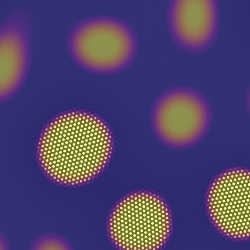
\includegraphics[width=\textwidth]{nucleation_and_sacrificial_growth}
        \label{fig:nucleation_and_growth}
        \caption{} 
    \end{subfigure}
    ~
    \begin{subfigure}[b]{0.3\textwidth}
        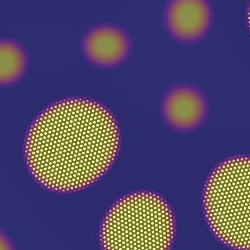
\includegraphics[width=\textwidth]{sacrificalgrowth}
        \label{fig:sacrifical_growth}
        \caption{}
    \end{subfigure}
    
    \vspace{0.5cm}
    \begin{subfigure}[b]{0.3\textwidth}
        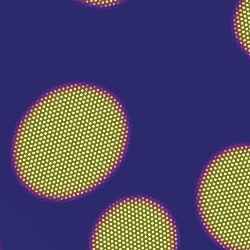
\includegraphics[width=\textwidth]{crystalgrowth}
        \label{fig:crystalgrowth}
        \caption{}
    \end{subfigure}
    ~
    \begin{subfigure}[b]{0.3\textwidth}
        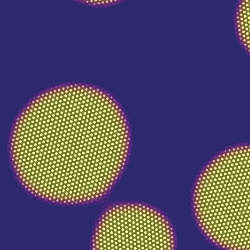
\includegraphics[width=\textwidth]{crystalgrowth2}
        \label{fig:crystalgrowth2}
        \caption{}
    \end{subfigure}
    ~ 
    \begin{subfigure}[b]{0.3\textwidth}
        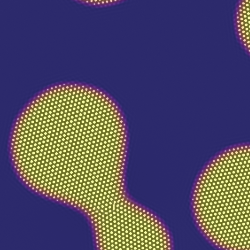
\includegraphics[width=\textwidth]{crystalgrowth3}
        \label{fig:crystalgrowth3}
        \caption{}
    \end{subfigure}
    \label{fig:preciptiation}
    \caption{Precipitation of nanoparticles from solution}
\end{figure}

\begin{figure}
    \centering
    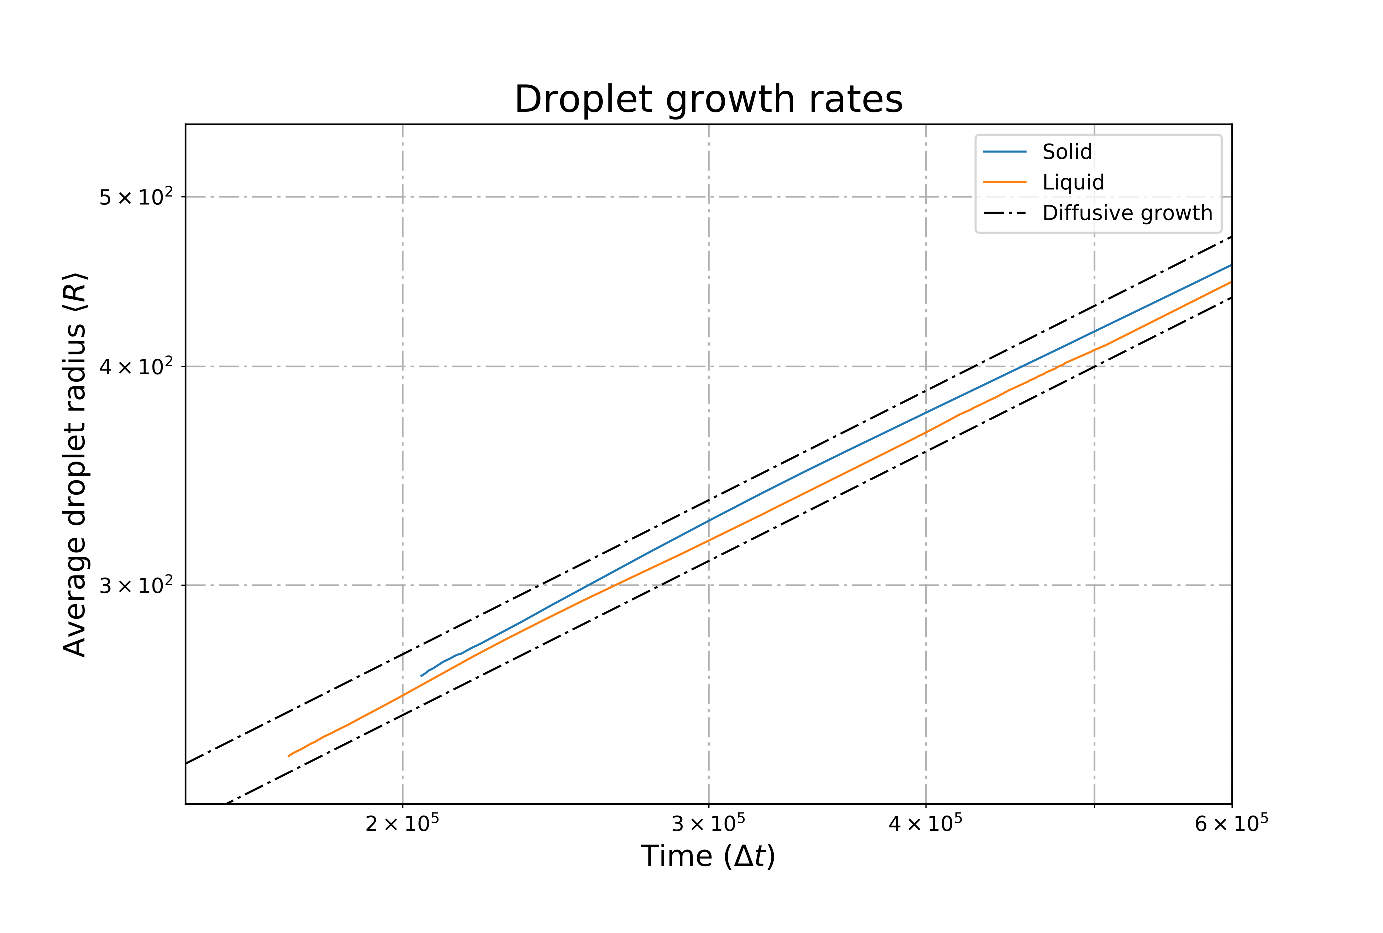
\includegraphics[width=\textwidth]{scaling}
    \label{fig:scaling}
    \caption{Droplet growth exponents}
\end{figure}

%%%%%%%%%%%%%%%%%%%%%%%%%%%%%%%
\section{Future Applications} %
%%%%%%%%%%%%%%%%%%%%%%%%%%%%%%%

